% file:         vlfeat.tex
% description:  An introduction to the VisionLab Features Library
% author:       Andrea Vedaldi

\documentclass{article}

\usepackage{graphicx}
\usepackage[margin=2cm]{geometry}
\usepackage{subfig}
\usepackage{xspace}
\usepackage{ifpdf}
\usepackage{visionlab}

\ifpdf
\DeclareGraphicsExtensions{.pdf,.eps,.png}
\usepackage{epstopdf}
\else
\DeclareGraphicsExtensions{.png,.eps,.pdf}
\fi

\newcommand{\VLFeat}{{\sc VLFeat}\xspace}
\title{An Introduction to the\\ VisionLab Features Library}
\author{Andrea Vedaldi \and Brian Fulkerson}

% --------------------------------------------------------------------
\begin{document}
% --------------------------------------------------------------------

\ifpdf\twocolumn\fi
\maketitle{}
\ifpdf\tableofcontents{}\fi

% --------------------------------------------------------------------
\section{Introduction}\label{intro}
% --------------------------------------------------------------------

\VLFeat (VisionLab Features Library) is a collection of computer
vision algorithms with a special focus on image features detection and
extraction such as SIFT and MSER. The core algorithms are implemented
in a lightweight and portable C-90 library (this library is documented
elsewhere and not covered by this article). The algorithms are made
accessible to the end user as command line and MATLAB programs.

This article provides a tutorial introduction to the main features of
\VLFeat. For a detailed description of the MATLAB and command line
utilites, the reader is referred to the relative built-in and
\verb$man$ documentation (respectively). For an overview of the
algorithms and their parameters, it is also reccomended to refer to
the documentation of the core library [].

% --------------------------------------------------------------------
\section{SIFT}\label{sift}
% --------------------------------------------------------------------

SIFT (scale-invariant feature transform) bundles a feature detector
and a feature descriptor.

\begin{figure*}
\subfloat[]{
\label{fig:sift-intro-a}
\includegraphics[width=0.32\textwidth]{figures/demo/sift_basic_0}}
\hfill
\subfloat[]{
\label{fig:sift-intro-b}
\includegraphics[width=0.32\textwidth]{figures/demo/sift_basic_2}}
\hfill
\subfloat[]{
\label{fig:sift-intro-c}
\includegraphics[width=0.32\textwidth]{figures/demo/sift_basic_3}}
\caption{{\em SIFT: frames and descriptors.} \subref{fig:sift-intro-a}
  a test image, \subref{fig:sift-intro-b} 50 detected features
  \subref{fig:sift-intro-c} and their
  descriptors.}\label{fig:sift-intro}
\end{figure*}

Both the detector and descriptor are accessible a single MATLAB
program \verb$sift$ (there is a similar command line utility). To
demonstrate the usage of \verb$sift$, we open MATLAB and we load a
test image (Fig.~\ref{fig:sift-intro-a}):
\begin{verbatim}
pfx = fullfile(vlfeat_root,'data','car1.jpg') ;
I = imread(pfx) ;
image(I) ;
\end{verbatim}
The \verb$sift$ command needs a gray scale image in single
precision. It also expects the image to be normalized in the $[0,255]$
range (although is not required, the default values of the various
thresholds used by the SIFT algorithm are tuned for this case). This
is obained by
\begin{verbatim}
I = float(rgb2gray(I)) ;
\end{verbatim}
We compute the SIFT frames (keypoints) and descriptors by
\begin{verbatim}
[f,d] = sift(I) ;
\end{verbatim}
The matrix \verb$f$ has a column for each frame with the parameters
$(x,y,\sigma,\theta)$. Here $(x,y)$ is the frame center, $\sigma$ the
frame scale (radius) and $\theta$ the frame ortientation. We visualize
a random selection of 50 features (Fig.~\ref{fig:sift-intro-b}) by:
\begin{verbatim}
perm = randperm(size(f,2)) ; 
sel  = perm(1:50) ;
h1   = plotframe(f(:,sel)) ; 
h2   = plotframe(f(:,sel)) ; 
set(h1,'color','y','linewidth',3) ;
set(h2,'color','k','linewidth',1) ;
\end{verbatim}
We can also overlay the descriptors (Fig.~\ref{fig:sift-intro-c}) by
\begin{verbatim}
h3 = plotsiftdescriptor(d(:,sel),f(:,sel)) ;  
set(h3,'color','g') ;
\end{verbatim}

% --------------------------------------------------------------------
\subsection{Detector parameters}\label{sift.parameters}
% --------------------------------------------------------------------

The SIFT detector is controlled mainly by two parameters: the peak
threshold and the (non) edge treshold. The {\bf peak treshold} filters
peaks of the DoG scale space that are too small (in absolute
value). For instance, consider the test image
(Fig.~\ref{fig:sift-peak-tresh}) obtained as a gradient of Gaussian
blobs:
\begin{verbatim}
I = double(rand(100,500) <= .005) ;
I = (ones(100,1) * linspace(0,1,500)) .* I ;
I(:,1) = 0 ; I(:,end) = 0 ;
I(1,:) = 0 ; I(end,:) = 0 ;
I = 2*pi*4^2 * imsmooth(I,4)
I = single(255 * I) ;
\end{verbatim}
We run the detector with peak treshold \verb$x$ by
\begin{verbatim}
f = sift(I, 'peaktresh', x) ;
\end{verbatim}
obtaining less and less features (Fig.~\ref{fig:sift-peak-tresh}).

\begin{figure}
\begin{center}
\includegraphics[width=0.9\columnwidth]{figures/demo/sift_peak_0}\\
\includegraphics[width=0.9\columnwidth]{figures/demo/sift_peak_1}\\
\includegraphics[width=0.9\columnwidth]{figures/demo/sift_peak_2}\\
\includegraphics[width=0.9\columnwidth]{figures/demo/sift_peak_3}\\
\includegraphics[width=0.9\columnwidth]{figures/demo/sift_peak_4}
\end{center}
\caption{{\em SIFT: peak treshold.} From top to bottom: test image and
  SIFT frames detected for increasing values of the peak treshold.}
\label{fig:sift-peak-tresh}
\end{figure}

The {\bf edge trehsold} instead eliminates peaks of the DoG scale
spcae whose curvature is below a certain treshold. The idea is that
such peaks are unstable because they are generated by edges and, as
such, do not yield stable feature frames. For instance, consider the etst
image (Fig.~\ref{fig:sift-edge-tresh})
\begin{verbatim}
I = zeros(100,500) ;
for i=[10 20 30 40 50 60 70 80 90]
  I(50-round(i/3):50+round(i/3),i*5) = 1 ;
end
I = 2*pi*8^2 * imsmooth(I,8) ;
I = single(255 * I) ;
\end{verbatim}
We run the detector with edge treshold \verb$x$ by
\begin{verbatim}
f = sift(I, 'peaktresh', x) ;
\end{verbatim}
obtaining more and more features (Fig.~\ref{fig:sift-edge-tresh}).

\begin{figure}
\begin{center}
\includegraphics[width=0.9\columnwidth]{figures/demo/sift_edge_0}\\
\includegraphics[width=0.9\columnwidth]{figures/demo/sift_edge_1}\\
\includegraphics[width=0.9\columnwidth]{figures/demo/sift_edge_2}\\
\includegraphics[width=0.9\columnwidth]{figures/demo/sift_edge_3}\\
\includegraphics[width=0.9\columnwidth]{figures/demo/sift_edge_4}
\end{center}
\caption{{\em SIFT: edge treshold.} From top to bottom: test image and
  SIFT frames detected for increasing values of the edge
  treshold. Notice that eventually, due to the interaction of nearby
  structures, some ``negative'' blobs are selected too.}
\label{fig:sift-edge-tresh}
\end{figure}


% --------------------------------------------------------------------
\subsection{Custom frames}\label{sift.custom}
% --------------------------------------------------------------------

The MATLAB command \verb$sift$ (and the command line utility) can
bypass the detector and run the descriptor on custom frames
(keypoints).
\begin{figure}
\begin{center}
\includegraphics[width=0.7\columnwidth]{figures/demo/sift_basic_4}
\end{center}
\caption{{\em SIFT: custom frames.} The descriptor computed at a
  custom frame.}
\label{fig:sift-custom}
\end{figure}
For instance, we can compute the descriptor of a SIFT frame centered
at position $(x,y)=(100,100)$, of scale $\sigma=10$ and orientation
$\theta=\pi/2$ (Fig~\ref{fig:sift-custom}) by
\begin{verbatim}
fc = [100;100;10;pi/8] ;
[f,d] = sift(I,'frames',fc) ;
\end{verbatim}
Mutiple frames \verb$fc$ an be specified as well. In this case they
are re-ordered by increasing scale.\footnote{The sorting anglorithm is
  stable, so the natural correspondence custom frames descriptors can
  be preserved by making sure to pass to the function a set of
  pre-predered frames.}


% --------------------------------------------------------------------
\section{MSER}\label{mser}
% --------------------------------------------------------------------


% --------------------------------------------------------------------
\appendix
\section{Overview of SIFT}\label{sift.overview}
% --------------------------------------------------------------------

This section gives a very quick overview of the SIFT detector and
descriptor. For details the reader is reccomended to refer to [].

\block{\bf Gaussian scale space and DoG.} SIFT starts by computing a
Gaussian scale space of the input image (Fig.~\ref{fig:sift-ss}). It
then computes second scale space, DoG (difference of Gaussians), by
subtracting successive layers of the Gaussian scale space.

\begin{figure}
\begin{center}
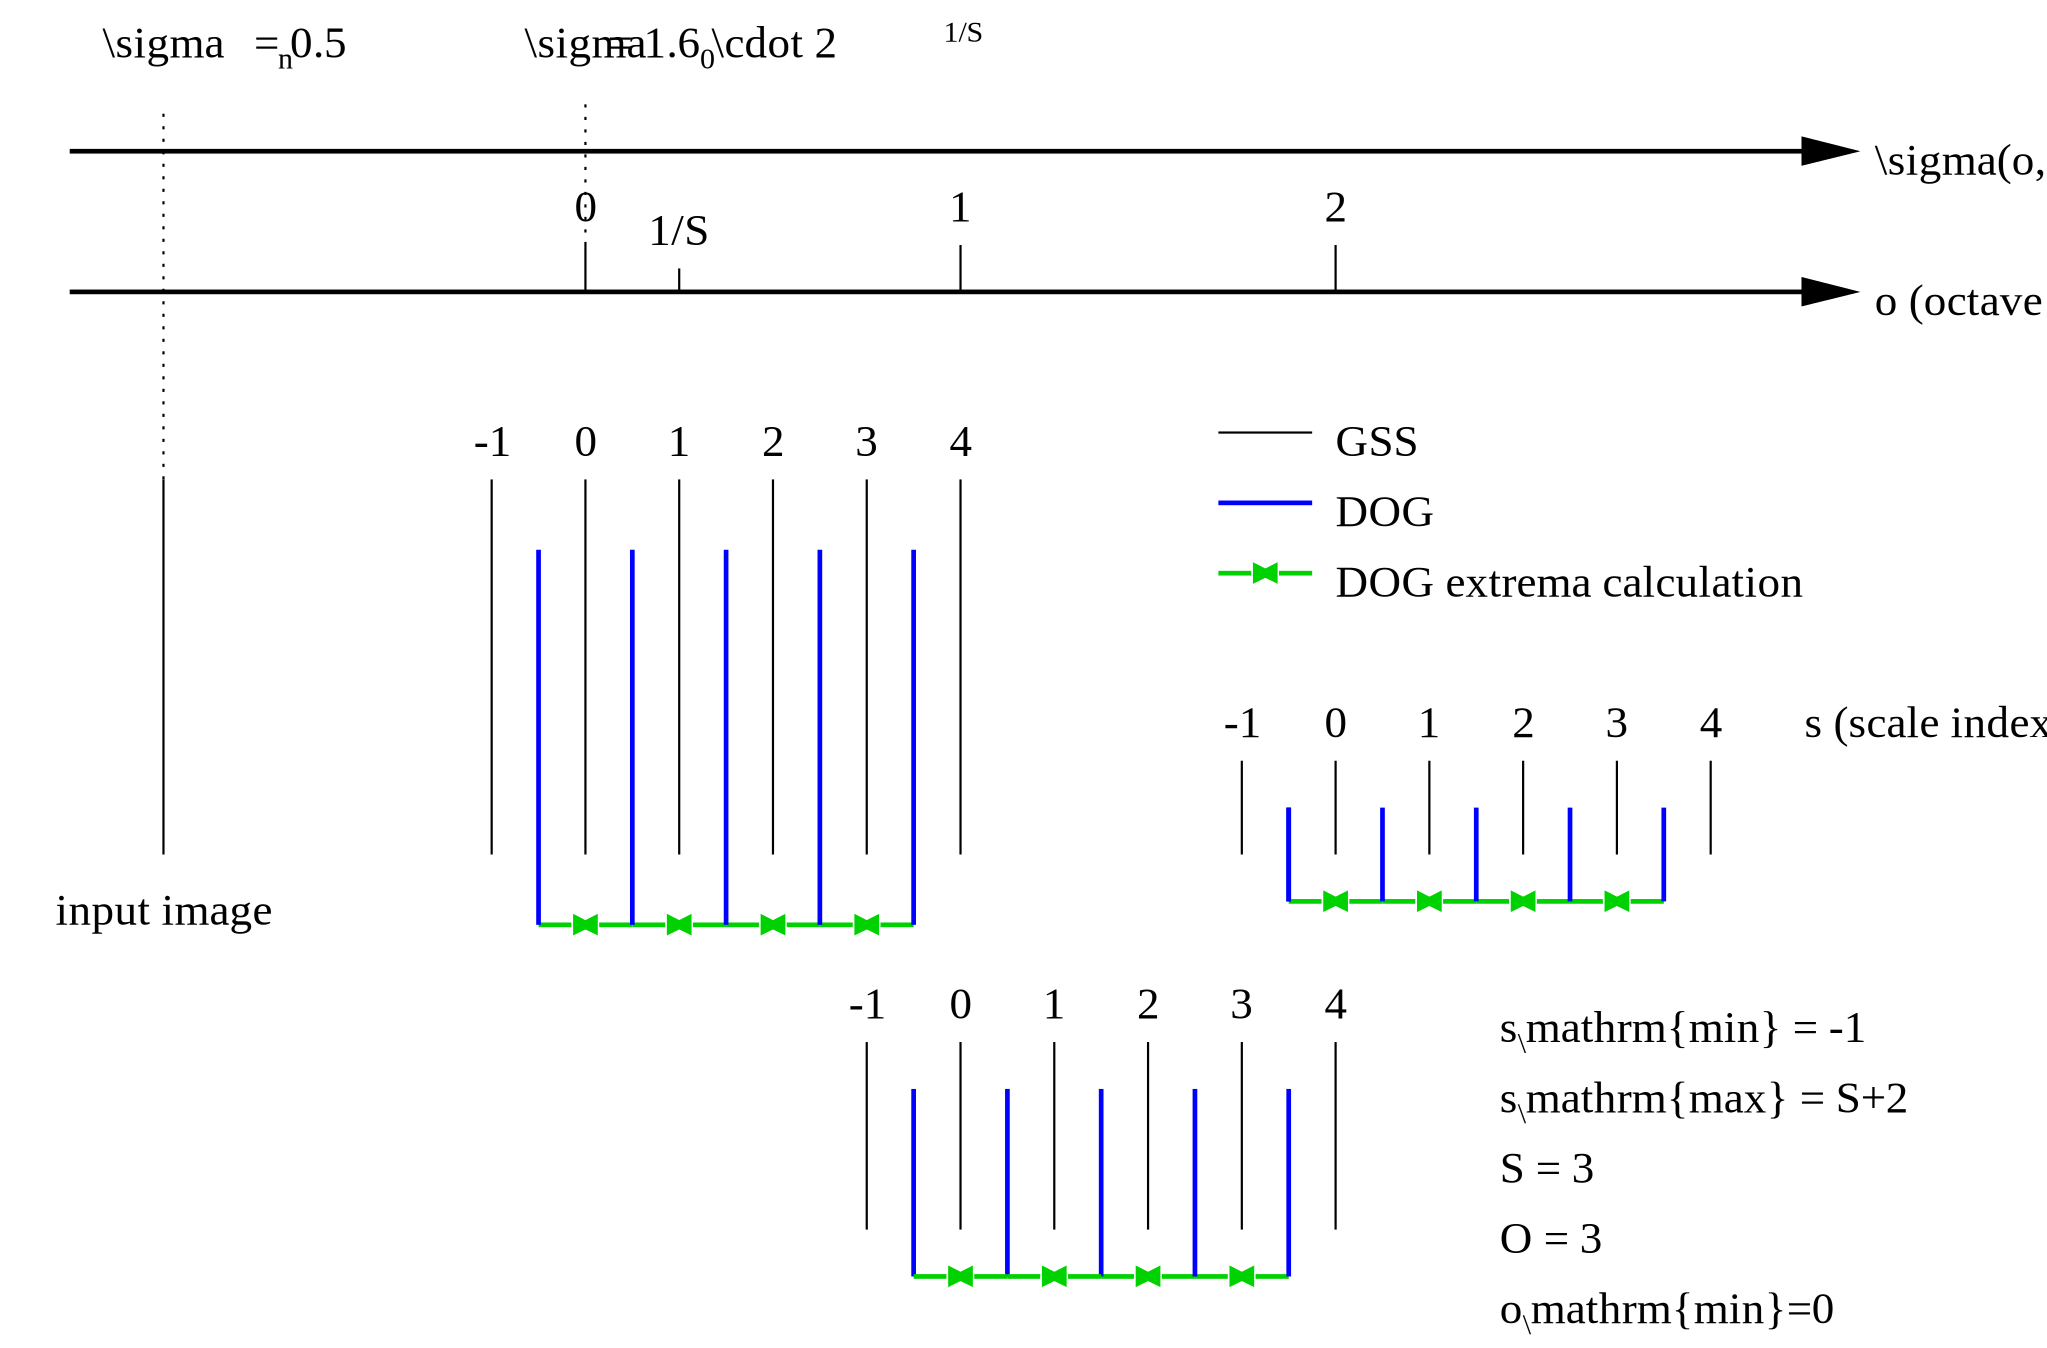
\includegraphics[width=\columnwidth]{figures/sift-ss}
\end{center}
\caption{{\em SIFT Scale Space.} From left to right, the input image
  $I$ is gradually convolved by Gaussian kernels of wider and wider
  variance and the resolution lowered. There are $O$ octaves and $S$
  levels per octave.}\label{fig:sift-ss}
\end{figure}

\block{\bf SIFT detector.} SIFT frames (keypoints) are selected as
local extrema of the DoG scale space (which is a 3-D
function). Unstable local extrema are filtered based on two
thresholds:
\begin{itemize}
\item {\em Peak threshold}. Extrema whose value is below this
  threshold are discared.
\item {\em Edge threshold}. The local curvature of the DoG function is
  evaluated and extrema whose curvature is below this threshold are
  discarded.
\end{itemize}

\block{\bf SIFT descriptor.} The SIFT descriptor is a 3-D histogram of
the local image gradient (Fig.~\ref{fig:sift-bins}).

\begin{figure}
\begin{center}
\includegraphics[width=\columnwidth]{figures/sift-bins}
\end{center}
\caption{{\em SIFT descriptor.} The SIFT descriptor is a 3-D histogram
  of the gradient orentations and positions of the local image
  patch. There are $N_o$ bins for the orientation and $N_p$ for each
  spatial direction. Binning is linearly interpolated and the gradient
  magnitude is weighed by a Gaussian window.}\label{fig:sift-bins}
\end{figure}

% --------------------------------------------------------------------
\end{document}
% --------------------------------------------------------------------